\documentclass[a4paper,twocolumn]{article}

\usepackage[left=1in, right=1in, top=0.5in, bottom=1in]{geometry}

\usepackage{siunitx}
\usepackage{hyperref}
\usepackage{circuitikz}
\usepackage{amsmath}
\usepackage{amsfonts}
\usepackage{mathtools}
\usepackage{physics}

\usepackage{import}
\usepackage{xifthen}
\usepackage{pdfpages}
\usepackage{transparent}

\newcommand{\incfig}[1]{
    \def\svgwidth{\columnwidth}
    \import{./figures/}{#1.pdf_tex}
}

\title{FP09 - Neuromorphic computing}
\author{R. Dorstijn (sd249) \& Moritz Epping (hh234)}
\date{December 2020}

\begin{document}
\maketitle

\section{Introduction}
\subsection{General theoretical background}
\subsubsection{Motivation}
Brains and computers often are compared because of their shared purpose,
decision making, though they have irreconcilable differences in architecture.
Modern computers function on the basis of the van Neumann
architecture\cite{von-Neumann}, which separates the control unit from the memory
and the computation unit. Though it simplifies the structure of the computer and
makes it modular, it does create a clear bottleneck at the communication layer,
commonly known as the von Neumann bottleneck. This creates an energy
inefficiency that is absolutely unacceptable for biological systems like that of
humans, who spend around 20\% of its total energy uptake on the brain\cite{metabolic-rates}.
This most likely has provided significant evolutionary pressure for hominids to
optimize metabolic resource usage\cite{seymour2016fossil}. For this reason a new
architecture for computers has been suggested: neuromorphic\footnote{``Neuro''
as in brain, ``-morphic'' as in having the shape of, forming ``having the shape
of a brain''.} computing.

\subsubsection{Signal processing in the brain}
Neurons (see fig \ref{fig:neuron}) are the basic computational components of the
brain, transmitting and morphing signals. Each neuron receives signals from
others at the dendrites, which shift the electric potential at the membrane of
the cell at the site of the synapse\footnote{The connection point of two
dendrites where the axon of one meets the dendrite of the other.}, creating an
ion wave crossing the entire membrane of the neuron, reaching it's axon,
allowing it to pass the signal on to other neurons.

\begin{figure}[ht]
    \centering
    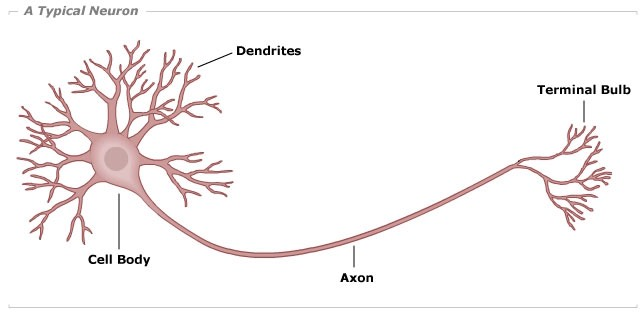
\includegraphics[width=.5\textwidth]{figures/neuron.jpg}
    \caption{Schematic image of a neuron, showing the dendrites, soma and axon.
    Source: Pennsylvania State University}
    \label{fig:neuron}
\end{figure}

The potential at the neuron membrane as a function of time is plotted in figure
\ref{fig:action-potential}, here it is demonstrated how a potential shift caused
by pre-synaptic\footnote{That is the neuron that passes on a signal to the
post-synaptic one.} neurons initiates a spike in the membrane potential, which
forces a release of ion containing vesicles at the terminal bulb, facilitating
the transfer of the signal by changing the relative potential at the dendrites.

\begin{figure}[ht]
    \centering
    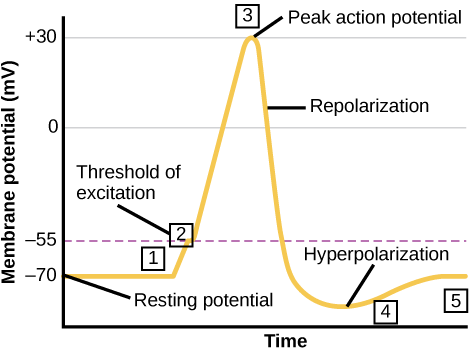
\includegraphics[width=.5\textwidth]{figures/action-potential.png}
    \caption{Formation of an action potential. Source:  \url{https://courses.lumenlearning.com/boundless-biology/chapter/how-neurons-communicate/}}
    \label{fig:action-potential}
\end{figure}

\subsubsection{The LIF model}
In order to emulate the behaviour electronically, a leaky integrate and fire
(LIF) model is used. A single neuron is represented by an electronic circuit
like the one in figure \ref{fig:circuit}. When the chip is not excited, nor
inhibited there is a constant ``leak'' voltage present on the membrane,
representing the biological rest potential of the membrane potential. When the
threshold voltage $V_\text{thres}$, the amplifier functioning as a comparator in
this setting, sends out a $V_{CC}$ signal to a digital unit that processes that
the neuron has fired and is responsible for closing the switch that keeps the
``membrane potential'' $V_m$ at some $V_\text{reset}$ for the refractory
period. This time is meant to mimic the period the voltage at the membrane
increases non-linearly and therefore loses its sensitivity to input. The digital
processing unit is also responsible for sending the signal (regardless of if it
is inhibitory or excitatory) to the neurons that the are connected to one that
just fired.

\begin{figure}[ht]
    \centering
    \begin{circuitikz}[scale = .6, transform shape]
        \draw (0, 0)    to node[midway, above]{$V_m$} (8.5, 0) node[op amp, anchor=+](A1){}; % main line
        \draw (A1.out)  to[short, l=$V_\text{out}$, -o] ++(1, 0);
        \draw (7, 1)    node[left, above] {$V_\text{thres}$} to[short, *-] (A1.-);
        \draw (0, 0)    to[vR, l=$g_l$, *-] (0, -2)
                        to[battery1, l=$E_l$] (0, -3) node[ground] {} (0, -4);
        \draw (2, 0)    to[vR, l=$g_x$, *-] (2, -2)
                        to[battery1, l=$E_x$] (2, -3) node[ground] {} (2, -4);
        \draw (4, 0)    to[vR, l=$g_i$, *-] (4, -2)
                        to[battery1, l=$E_g$] (4, -3) node[ground] {} (4, -4);
        \draw (6, 0)    to[C, l=$C_m$] (6, -2)
                        node[ground] {} (6, -2);
        \draw (7.5, -2) node[anchor=north] {$V_\text{reset}$}
                        to[short, o-] (7.5, -1)
                        to[normal open switch, -*] (7.5, 0);
        \draw [densely dashed]
              (3.3, -4) --++(0, 4.6)
                        --++(5, 0)
                        --++(0, -4.6)
                        --++(-5, 0);
    \end{circuitikz}
    \caption{Circuit of a single neuron in a LIF chip.}
    \label{fig:circuit}
\end{figure}

\subsection{Background for the experiments}
\subsubsection{Investigation of a single neuron}
A single neuron will be investigated, without considering any excitatory or
inhibitory influences. This simplifies the circuit of figure \ref{fig:circuit}
to the diagram in figure \ref{fig:circuit-simplified}. The relevant parameters
that appear from this figure are:

\begin{figure}[hb]
    \centering
    \begin{circuitikz}
        \draw (0, 0)    node[ground] {}
                        to[battery1, l=$E_l$]       ++(0, 2)
                        to[vR, l=$g_l$]             ++(2, 0)
                        to[C, l=$C_m$]              ++(2, 0)
                        to[short]                   ++(0, -1)
                        node[ground] {};
        \draw (-2, 0)   node[below] {$V_\text{reset}$}
                        to[normal open switch, o-]  ++(0, 2)
                        to[short, -*]               ++(2, 0);
    \end{circuitikz}
    \caption{Circuit in figure \ref{fig:circuit} simplified for the scenario
    that no signals are incoming for this particular neuron.}
    \label{fig:circuit-simplified}
\end{figure}

\begin{itemize}
    \item $E_l$ setting the \textit{amount} of potential leaking into the `membrane'.
    \item $g_l$ determining how \textit{quickly} the potential leaks into the `membrane'.
    \item $C_m$ describing how much potential is leaked to ground.
    \item $V_\text{reset}$ prescribing the starting point of a cycle.
\end{itemize}

The last item in this list hints at that we do not yet know when the cycle will
end. In the previous section it was stated that $V_\text{thres}$ determines
this value. With this last variable in place it will now be possible to
reconstruct the entire charging and resetting of the $V_m$, this period will be
called $\tau_m$.

However one item is missing: the refraction period. Recall that this is the
period in which the neuron is `off' and does not take in input. Meaning that
this time should be accounted for when calculating the total period.
\begin{equation}
    \tau = \tau_m + \tau_\text{refrac}
    \label{eq:tau}
\end{equation}

\subsubsection{Calibrating neuron parameters}
In the case of a single unconnected neuron the membrane potential can be
understood with application of the Kirchoff formula to the circuit in figure
\ref{fig:circuit-simplified}.
\[
    C_m \frac{dV_m}{dt} = g_l(E_l - V_m)
\]
Clearly, this is a ordinary first order differential equation and has the
solution
\begin{equation}
    V_m(t) = A \exp(\frac{-g_l}{C_m}t) - E_l
    \label{eq:diff-eq-sol}
\end{equation}
where $A$ is given by the initial condition:
\[
    A = V_m(0) - E_l.
\]

In order to set a neuron to fire at a regular frequency $\tau_m$, we have to take
into account that $V_m$ will be reset to $V_\text{reset}$ when it hits
$V_\text{thres}$. Equation \eqref{eq:diff-eq-sol} can be rephrased in terms of
$t$.
\[
    \tau_m = -\ln(\frac{V_\text{thres} - E_l}{V_\text{reset} - E_l})
    \frac{C_m}{g_l}
\]

The characteristic time constant $\tau_c$ of the system can be found by setting
$V_\text{thres}$ as a function of $E_l$ and $V_\text{reset}$.
\[
    V_\text{thres} = E_l - (E_l - V_\text{reset})\exp(-1)
\]
The resulting $\tau_c$ is then only dependent on $C_m$ and $g_l$:
\begin{align*}
    \tau_m &= -\ln(\frac{E_l - (E_l - (E_l - V_\text{reset})\exp(-1))}{V_\text{reset} - E_l}) \frac{C_m}{g_l}\\
           &= -\ln(\frac{(E_l - V_\text{reset})\exp(-1))}{V_\text{reset} - E_l})\frac{C_m}{g_l} \\
           &= \frac{C_m}{g_l} = \tau_c
\end{align*}
This time constant does not take into account the refractory period which should
adds a fixed contribution. This was mentioned in equation \eqref{eq:tau}, but
becomes relevant again when considering the total time.

This describes a good theory of the neuron, however in reality there are some
serious production artifacts that require calibration.

\subsubsection{A Single Neuron with Synaptic Input}
\subsubsection{Short Term Plasticity}
\subsubsection{Feed-Forward Networks}
One of the simplest neural networks one can consider is the feed-forward
network in which every neuron is arranged so that it passes on the signal it
receives to the next. In nature, a single neuron firing has relatively little
meaning until it is put in a larger context. Most of these contexts can be
simplified by viewing them as `superpositions' feed forward networks. It is
however important to consider that in nature robustness and redundancy is
highly favored in critical systems. The function of a feed-forward network can
be shutdown entirely if one neuron fails for whatever reason. Hence the concept
of populations is introduced, these are groups of neurons that perform the same
logical operations\footnote{That is to say, they are all either inhibitory or
excitatory neurons, they have the same neurons as inputs and the share the same
output neurons.} This is visualized in figure \ref{fig:feed-forward}.

\begin{figure}[ht]
    \centering
    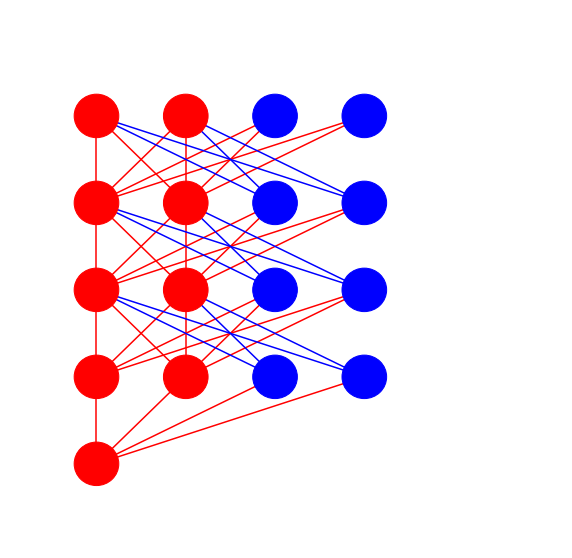
\includegraphics[width=.5\textwidth]{figures/feedforward network.png}
    \caption{Feed forward network with length 4 and population size 2. Two input
        neurons are drawn additionally. Exhibitory neurons and connections are drawn
        in red, inhibitory ones in blue.}
    \label{fig:feed-forward}
\end{figure}

In this experiment, connection weights also become relevant for the first time.
Any synaptic connection is assigned a weight, this weight represents the
membrane potential increase that a signal transfer induces. The importance of
this variable is crucial for networks as it nearly completely describes the
behaviour of a network.

\subsubsection{Recurrent Networks}
\subsubsection{A Simple Computation: XOR}

\section{Execution \& Results}
A rather interesting setup was provided by the university of Heidelberg. It
hosted a SPIKEY chip on its grounds, which was physically inaccessible due to
the COVID-19 crisis, therefore it was connected to a job manager that could be
written to by the Jülich Supercomputing Center, which hosted Jupyter notebooks
for this purpose. A SPIKEY chip implements the LIF model physically.

\subsection{Investigation of a single neuron}
% Moritz does this part
\subsubsection{Setup/Settings}
\subsubsection{Results}

\subsection{Calibrating neuron parameters}
On the SPIKEY chip 4 neurons were isolated programmatically and given the same
parameters:
\begin{itemize}
    \item $V_\text{reset}$: \SI{-80.0}{\milli\volt}
    \item $V_\text{thresh}$: \SI{-55.0}{\milli\volt}
    \item $E_\text{leak}$: \SI{-50.0}{\milli\volt}
    \item $g_\text{leak}$:  \SI{20.0}{\nano\siemens}
\end{itemize}

This however resulted in wildly differing frequencies, as becomes visible in
figure \ref{fig:4membranes}. In order to compensate for this $g_l$ was adjusted
individually for all of the membranes so that they were all correct within their
respective standard deviation: \SI{20.1}{\milli\volt}, \SI{55.0}{\milli\volt},
\SI{60.0}{\milli\volt}, \SI{20.5}{\milli\volt}.

\begin{figure}[ht]
    \centering
    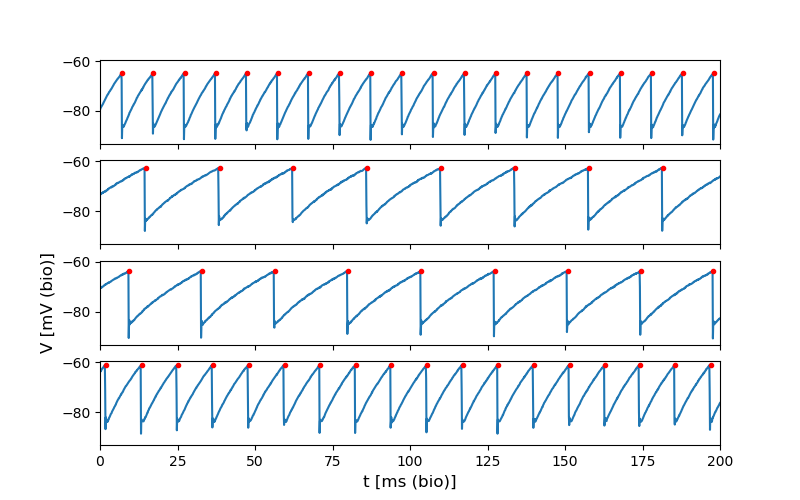
\includegraphics[width=.5\textwidth]{figures/4membranes.png}
    \caption{Biological membrane potential of four membranes with the same
    setting. The red dots indicate when the digital processing units recognizes
    that voltage reaches the threshold. The rates for the signals are
    \SI{1.02(2)e1}{\milli\second}, \SI{2.41(3)e1}{\milli\second},
    \SI{2.36(1)e1}{\milli\second}, \SI{1.15(1)e1}{\milli\second}, in the same
    order that they presented in the image. }
    \label{fig:4membranes}
\end{figure}

The scale of the problem becomes even more clear when considering the that one
half of the SPIKEY chip has a rate distribution like presented in figure
\ref{fig:distribution}, the previous method of trial and error becomes rather
infeasible.

\begin{figure}[ht]
    \centering
    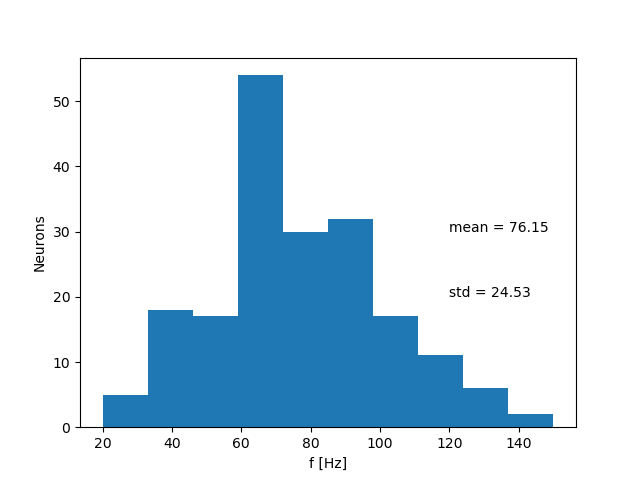
\includegraphics[width=.5\textwidth]{figures/rate-distribution.png}
    \caption{Distribution of firing rate for the same across one side of the
    chip.}
    \label{fig:distribution}
\end{figure}

Instead an algorithm is suggested that should help find a proper calibration for
all neurons that are able to converge on the desired rate.
\begin{enumerate}
    \item Set the $g_l$ to the default value and measure the rate of the neuron.
    \item Set the $g_l$ to double the default value and measure the rate of the
        neuron.
    \item Describe the response of the neuron linearly using the last two
        points and estimate where the desired rate would lie.
    \item Set the $g_l$ to this value and measure the rate, if it is within the
        standard error: success! If not return to step 3.
\end{enumerate}
Sadly we were unable to implement the algorithm, but we encourage the reader
to.

\subsection{A Single Neuron with Synaptic Input}
\subsection{Short Term Plasticity}

\subsection{Feed-Forward Networks}
A feed-forward network is described by the population number, the chain length
(see figure \ref{fig:feed-forward}) and the several weights of the following
type connections:
\begin{itemize}
    \item From the initial excitatory neuron to the first excitatory member of the
        chain. (ex0 $\rightarrow$ ex)
    \item From the initial excitatory neuron to the first inhibitory member of the
        chain. (ex0 $\rightarrow$ inh)
    \item From an excitatory neuron in the chain to the next excitatory neuron.
        (ex $\rightarrow$ ex)
    \item From an excitatory neuron in the chain to the next inhibitory neuron.
        (ex $\rightarrow$ inh)
    \item From an inhibitory neuron in the chain to the next excitatory neuron.
        (inh $\rightarrow$ ex)
\end{itemize}
This coincidentally is also the order of sensitivity (top being most sensitive),
particularly when discussing the `width' of the signal. With this is meant the
the amount of consequent signals that follow a single input signal. When having
a large population, a high (inh $\rightarrow$ ex) wheight was capable of
stopping the signal before it would reach the last neuron.

An issue that occurred as the chain length was increased the width of the signal
did as well. A length of 60 was reached creating a width of 10. This worked for
low populations, however with higher populations the membrane voltage was
overall raised to such a degree that the neurons started firing randomly and the
signal was lost. The theoretical maximum amount of neurons that could be used in
a chain is 192, so that for a population of size $n$ the max chain length
$c_\text{max}$ would be $c_\text{max} = 192 / n$.

An interesting phenomena occurs when the network is configured to loop. That is
to say the last neuron excites the first. Sadly it was not possible to set the
signal delay, which would have allowed for more careful investigation, but still
there was a clear effect visible in figure \ref{fig:feed-forward-loop}.

\begin{figure}
    \centering
    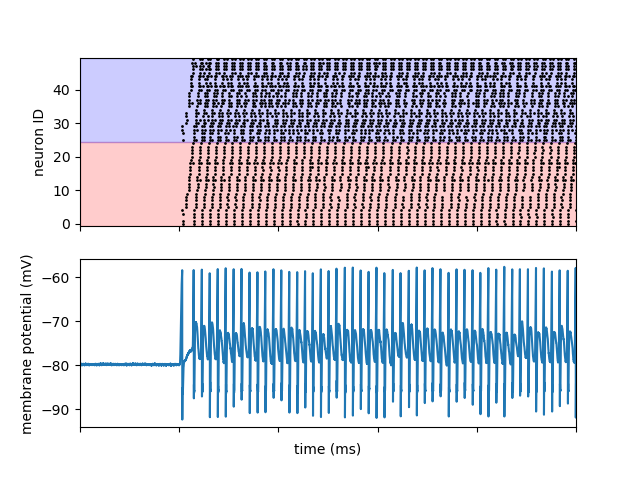
\includegraphics[width=.5\textwidth]{figures/feedforward signals loop.png}
    \caption{Feed-forward network configured in a loop. The population is 5, as
        is the chain length. Note that at the end the width starts to increase.
        The top figure shows all signals send by the neurons. The blue area
        represents inhibitory neurons, the red excitatory. The bottom figure
        shows the membrane potential of the first excitatory neuron.}
    \label{fig:feed-forward-loop}
\end{figure}

\subsection{Recurrent Networks}
\subsection{A Simple Computation: XOR}

\bibliography{main}
\bibliographystyle{ieeetr}

\section{Appendix}
% Notebook PDFs here

\end{document}
